\chapter*{Instructions to Authors}
\label{authorguide}

\paragraph{Audience}
Refer to the \emph{Author-Audience Matrix}.
Identify which row (or rows, for mixed groups of co-authors) you inhabit, and then make a choice of which audience your article will address.
We encourage you to share lessons and insights which are broadly reusable (i.e. cover two or more points), but it is critical that \emph{ELR} editors are able to discern your choice.
Either note your audience choice when submitting, or make some explicit reference to it in your text.
\begin{figure}
\centering
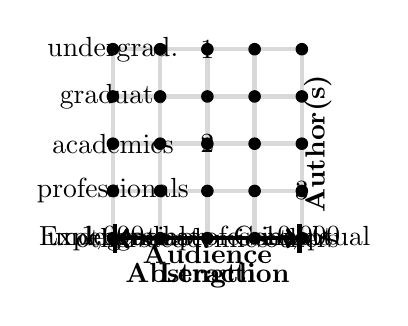
\begin{tikzpicture}[pubaxis/.style={font=\bfseries\scshape}]
  \draw[draw=gray!30,ultra thick,step=6mm] (0,0) grid (24mm,24mm);
  \foreach \x in {0,6,...,24}
    \foreach \y in {0,6,...,24}
      \fill (\x mm,\y mm) circle (0.8mm);
  \path;
  { [every node/.style={anchor=north west,scale=0.8}]
    \node at (12mm,24mm) {1};
    \node at (12mm,12mm) {2};
    \node at (24mm,6mm) {3};
  }
  { [every node/.style={inner sep=3mm}]
    { [shift={(0,24mm)},every node/.style={anchor=base west,rotate=60}]
      \node at (0,0) {undergrad.};
      \node at (6mm,0) {graduate};
      \node at (12mm,0) {academics};
      \node at (18mm,0) {professionals};
      \node at (24mm,0) {others};
    }
    { [every node/.style={anchor=mid east}]
      \node at (0,24mm) {undergrad.};
      \node at (0,18mm) {graduate};
      \node at (0,12mm) {academics};
      \node at (0,6mm) {professionals};
      \node at (0,0) {others};
    }
    { [every node/.style={anchor=north}]
      \node [pubaxis,rotate=90] at (26mm,12mm) {Author(s)};
      \node [pubaxis] at (12mm,-2mm) {Audience};
    }
  }
  { [shift={(42mm,3mm)}]
    \draw [|<->|,ultra thick] (0,0) -- (24mm,0);
    \node [pubaxis,anchor=north] at (12mm,-2mm) {Length};
    { [every node/.style={anchor=south,inner sep=3mm,scale=0.8}]
      \node at (0,0) {1,000};
      \node at (24mm,0) {10,000};
    }
  }
  { [shift={(42mm,18mm)}]
    \draw [|<->|,ultra thick] (0,0) -- (24mm,0);
    \node [pubaxis,anchor=north] at (12mm,-2mm) {Abstraction};
    { [every node/.style={anchor=south,inner sep=3mm,scale=0.8}]
      \node at (0,0) {Experiential};
      \node at (24mm,0) {Conceptual};
    }
  }
\end{tikzpicture}
\caption{Author-Audience Matrix. \textbf{(1)} includes student coursework, \textbf{(2)} includes most technical journals, and \textbf{(3)} could be engineering consultants reporting to a client firm.}
\end{figure}

\paragraph{Format, length \& language}
Choose a target length in increments of 500 words.
1000 words is a rough (but not absolute) minimum.
\emph{ELR} prefers long-format writing; give your whole thoughts, not just sketches of them.

\emph{ELR} accepts submissions in Canadian English and French.

\paragraph{Reviews \& revisions}
Articles are subject to double-blind reviews; the author(s) are anonymous to the reviewers and vice versa.
Where possible the reviewers will be from the audience chosen by the author(s).
Reviewers have the option to recommend an article be resubmitted for review, in which case a second review is undertaken after revisions have taken place.
Otherwise an \emph{ELR} Section Editor will coordinate revisions with author(s) and recommend acceptance to the Editorial Board once (s)he judges the reviewer's concerns are satisfied.

\paragraph{Technical}

